% Options for packages loaded elsewhere
\PassOptionsToPackage{unicode}{hyperref}
\PassOptionsToPackage{hyphens}{url}
\PassOptionsToPackage{dvipsnames,svgnames,x11names}{xcolor}
%
\documentclass[
  letterpaper,
  DIV=11,
  numbers=noendperiod]{scrartcl}

\usepackage{amsmath,amssymb}
\usepackage{iftex}
\ifPDFTeX
  \usepackage[T1]{fontenc}
  \usepackage[utf8]{inputenc}
  \usepackage{textcomp} % provide euro and other symbols
\else % if luatex or xetex
  \usepackage{unicode-math}
  \defaultfontfeatures{Scale=MatchLowercase}
  \defaultfontfeatures[\rmfamily]{Ligatures=TeX,Scale=1}
\fi
\usepackage{lmodern}
\ifPDFTeX\else  
    % xetex/luatex font selection
\fi
% Use upquote if available, for straight quotes in verbatim environments
\IfFileExists{upquote.sty}{\usepackage{upquote}}{}
\IfFileExists{microtype.sty}{% use microtype if available
  \usepackage[]{microtype}
  \UseMicrotypeSet[protrusion]{basicmath} % disable protrusion for tt fonts
}{}
\makeatletter
\@ifundefined{KOMAClassName}{% if non-KOMA class
  \IfFileExists{parskip.sty}{%
    \usepackage{parskip}
  }{% else
    \setlength{\parindent}{0pt}
    \setlength{\parskip}{6pt plus 2pt minus 1pt}}
}{% if KOMA class
  \KOMAoptions{parskip=half}}
\makeatother
\usepackage{xcolor}
\setlength{\emergencystretch}{3em} % prevent overfull lines
\setcounter{secnumdepth}{5}
% Make \paragraph and \subparagraph free-standing
\makeatletter
\ifx\paragraph\undefined\else
  \let\oldparagraph\paragraph
  \renewcommand{\paragraph}{
    \@ifstar
      \xxxParagraphStar
      \xxxParagraphNoStar
  }
  \newcommand{\xxxParagraphStar}[1]{\oldparagraph*{#1}\mbox{}}
  \newcommand{\xxxParagraphNoStar}[1]{\oldparagraph{#1}\mbox{}}
\fi
\ifx\subparagraph\undefined\else
  \let\oldsubparagraph\subparagraph
  \renewcommand{\subparagraph}{
    \@ifstar
      \xxxSubParagraphStar
      \xxxSubParagraphNoStar
  }
  \newcommand{\xxxSubParagraphStar}[1]{\oldsubparagraph*{#1}\mbox{}}
  \newcommand{\xxxSubParagraphNoStar}[1]{\oldsubparagraph{#1}\mbox{}}
\fi
\makeatother


\providecommand{\tightlist}{%
  \setlength{\itemsep}{0pt}\setlength{\parskip}{0pt}}\usepackage{longtable,booktabs,array}
\usepackage{calc} % for calculating minipage widths
% Correct order of tables after \paragraph or \subparagraph
\usepackage{etoolbox}
\makeatletter
\patchcmd\longtable{\par}{\if@noskipsec\mbox{}\fi\par}{}{}
\makeatother
% Allow footnotes in longtable head/foot
\IfFileExists{footnotehyper.sty}{\usepackage{footnotehyper}}{\usepackage{footnote}}
\makesavenoteenv{longtable}
\usepackage{graphicx}
\makeatletter
\newsavebox\pandoc@box
\newcommand*\pandocbounded[1]{% scales image to fit in text height/width
  \sbox\pandoc@box{#1}%
  \Gscale@div\@tempa{\textheight}{\dimexpr\ht\pandoc@box+\dp\pandoc@box\relax}%
  \Gscale@div\@tempb{\linewidth}{\wd\pandoc@box}%
  \ifdim\@tempb\p@<\@tempa\p@\let\@tempa\@tempb\fi% select the smaller of both
  \ifdim\@tempa\p@<\p@\scalebox{\@tempa}{\usebox\pandoc@box}%
  \else\usebox{\pandoc@box}%
  \fi%
}
% Set default figure placement to htbp
\def\fps@figure{htbp}
\makeatother

\usepackage{booktabs}
\usepackage{longtable}
\usepackage{array}
\usepackage{multirow}
\usepackage{wrapfig}
\usepackage{float}
\usepackage{colortbl}
\usepackage{pdflscape}
\usepackage{tabu}
\usepackage{threeparttable}
\usepackage{threeparttablex}
\usepackage[normalem]{ulem}
\usepackage{makecell}
\usepackage{xcolor}
\KOMAoption{captions}{tableheading}
\makeatletter
\@ifpackageloaded{caption}{}{\usepackage{caption}}
\AtBeginDocument{%
\ifdefined\contentsname
  \renewcommand*\contentsname{Table of contents}
\else
  \newcommand\contentsname{Table of contents}
\fi
\ifdefined\listfigurename
  \renewcommand*\listfigurename{List of Figures}
\else
  \newcommand\listfigurename{List of Figures}
\fi
\ifdefined\listtablename
  \renewcommand*\listtablename{List of Tables}
\else
  \newcommand\listtablename{List of Tables}
\fi
\ifdefined\figurename
  \renewcommand*\figurename{Figure}
\else
  \newcommand\figurename{Figure}
\fi
\ifdefined\tablename
  \renewcommand*\tablename{Table}
\else
  \newcommand\tablename{Table}
\fi
}
\@ifpackageloaded{float}{}{\usepackage{float}}
\floatstyle{ruled}
\@ifundefined{c@chapter}{\newfloat{codelisting}{h}{lop}}{\newfloat{codelisting}{h}{lop}[chapter]}
\floatname{codelisting}{Listing}
\newcommand*\listoflistings{\listof{codelisting}{List of Listings}}
\makeatother
\makeatletter
\makeatother
\makeatletter
\@ifpackageloaded{caption}{}{\usepackage{caption}}
\@ifpackageloaded{subcaption}{}{\usepackage{subcaption}}
\makeatother

\usepackage{bookmark}

\IfFileExists{xurl.sty}{\usepackage{xurl}}{} % add URL line breaks if available
\urlstyle{same} % disable monospaced font for URLs
\hypersetup{
  pdftitle={Supplementary Materials of Impact of IPTp Regimen on Pregnancy Outcomes},
  pdfauthor={Asmith Joseph},
  colorlinks=true,
  linkcolor={blue},
  filecolor={Maroon},
  citecolor={Blue},
  urlcolor={Blue},
  pdfcreator={LaTeX via pandoc}}


\title{Supplementary Materials of Impact of IPTp Regimen on Pregnancy
Outcomes}
\author{Asmith Joseph}
\date{}

\begin{document}
\maketitle


\newpage{}

\section{Overview}\label{overview}

The Supplementary Appendix begins with comprehensive methodological
details, including variable‐by‐variable missingness (Table S1), analysis
of deviance comparing models with and without the malaria×SP interaction
(Table S2), and variance inflation factors for the final interaction
model (Table S3). It also presents machine‐learning tuning results with
the top five elastic-net hyperparameter combinations ranked by mean
cross-validated AUC (Table S4) alongside a heatmap illustrating AUC
across the penalty--mixture grid (Figure S1). Full code excerpts
document our data-cleaning steps, rsample splits, recipe definitions,
and tune\_grid workflows. The appendix then moves on to additional
results: a detailed stratification of outcome measures and
malaria-exposure variables by IPTp arm (Table S5), bar graphs of total
malaria episodes during pregnancy (Figure S2), gravidity (Figure S3),
and parity (Figure S4) distributions by treatment arm, and a bootstrap
calibration curve for the interaction model (Figure S5). Finally, it
compares model discrimination with overlaid ROC curves for logistic
regression, random forest, and XGBoost (Figure S6), presents a
precision-recall curve for the top‐performing machine-learning model
(Figure S7), and reports the test-set AUC for the gravidity-only model
in women under 25 years (Table S6).

~ ~

\section{Code and file information}\label{code-and-file-information}

The Supplementary Appendix is built with a clear, step‑wise workflow:
raw PROMO trial data are first cleaned and documented, then transformed
into the analysis dataset. Subsequent scripts generate missingness
tables, interaction model diagnostics, machine‑learning tuning results,
and additional stratified analyses. Each RMarkdown file lives in the
code/ subfolders (processing, EDA, analysis), reads from data/, and
writes results into results/. Finally, the Quarto source in
products/manuscript/supplement renders the assembled tables and figures
into Supplementary‑Material.docx. Running the scripts in their numeric
order fully reproduces every table and figure in this appendix.

\subsection{📁 Directory Structure
Overview}\label{directory-structure-overview}

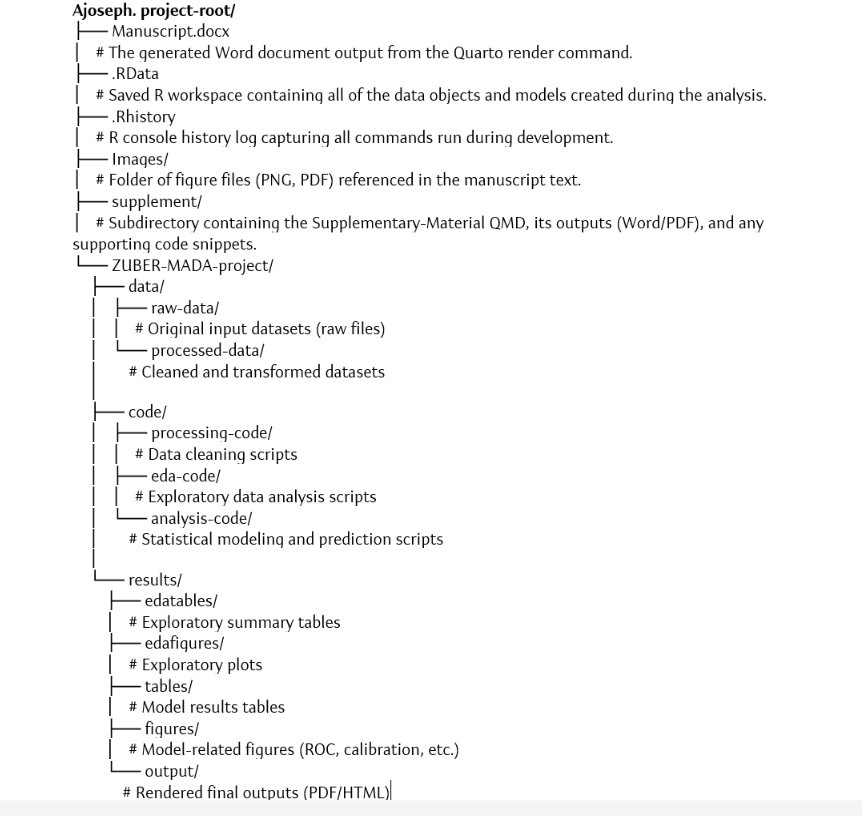
\includegraphics[width=2.39in,height=\textheight,keepaspectratio]{../Images/Project-root.png}

\newpage{}

\section{Additional results}\label{additional-results}

\section{\# Exploratory Analysis: Malaria Episodes, Gravidity/Parity,
and Treatment
Arm}\label{exploratory-analysis-malaria-episodes-gravidityparity-and-treatment-arm}

The four supplementary EDA plots concisely overview key baseline
characteristics by treatment arm and the height--weight relationship at
enrollment. The first panel shows that the majority of women experienced
one malaria episode during pregnancy, with progressively fewer in the
2--3 and ≥4 categories and that counts are consistently higher in the DP
arm than the SP arm across all episode bins. The second panel depicts
gravidity stratified into 1, 2--3, and ≥4 pregnancies, revealing a
similar pattern in both arms but a noticeably smaller proportion of
primigravidae in the SP group. The third panel presents parity
categories (0, 1--2, ≥3), again demonstrating broadly comparable
distributions between arms, with a slight excess of women with ≥3
previous births in the DP arm. Finally, the scatterplot of maternal
height and weight, with a LOESS smoothing curve and 95\% confidence
band, confirms a modest positive association between height and weight
at enrollment, supporting the use of both measures in downstream
modeling.

\emph{Figure S1.Total Malaria Episodes During Pregnancy by Treatment
Arm}

\pandocbounded{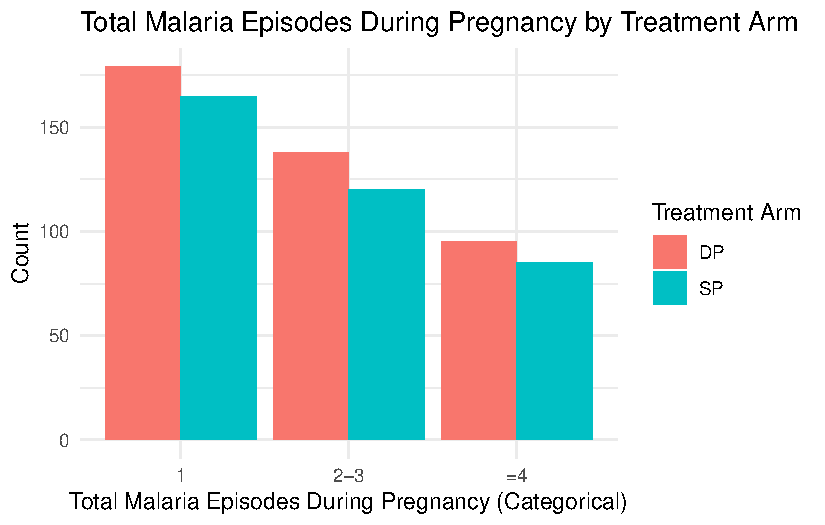
\includegraphics[keepaspectratio]{Supplementary-Material_files/figure-pdf/unnamed-chunk-4-1.pdf}}

~ ~

\emph{Figure S2: Gravidity Distribution by Treatment Arm}

\pandocbounded{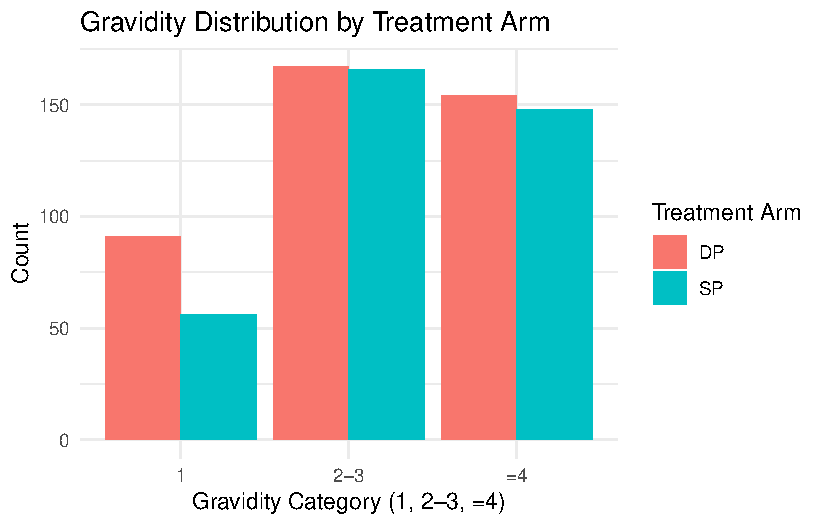
\includegraphics[keepaspectratio]{Supplementary-Material_files/figure-pdf/unnamed-chunk-5-1.pdf}}

~ ~

\emph{Figure S3: Parity Distribution by Treatment Arm}

\pandocbounded{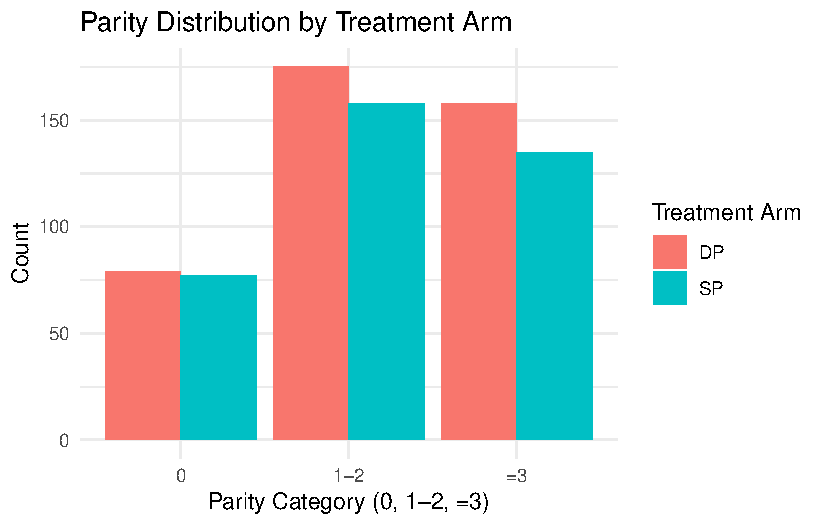
\includegraphics[keepaspectratio]{Supplementary-Material_files/figure-pdf/unnamed-chunk-6-1.pdf}}

~ ~

\emph{Figure S4:Scatterplot of maternal weight by height with fitted
LOESS smoothing curve (95\% CI) --- exploratory assessment of the
height--weight relationship at enrollment}

\begin{figure}

\centering{

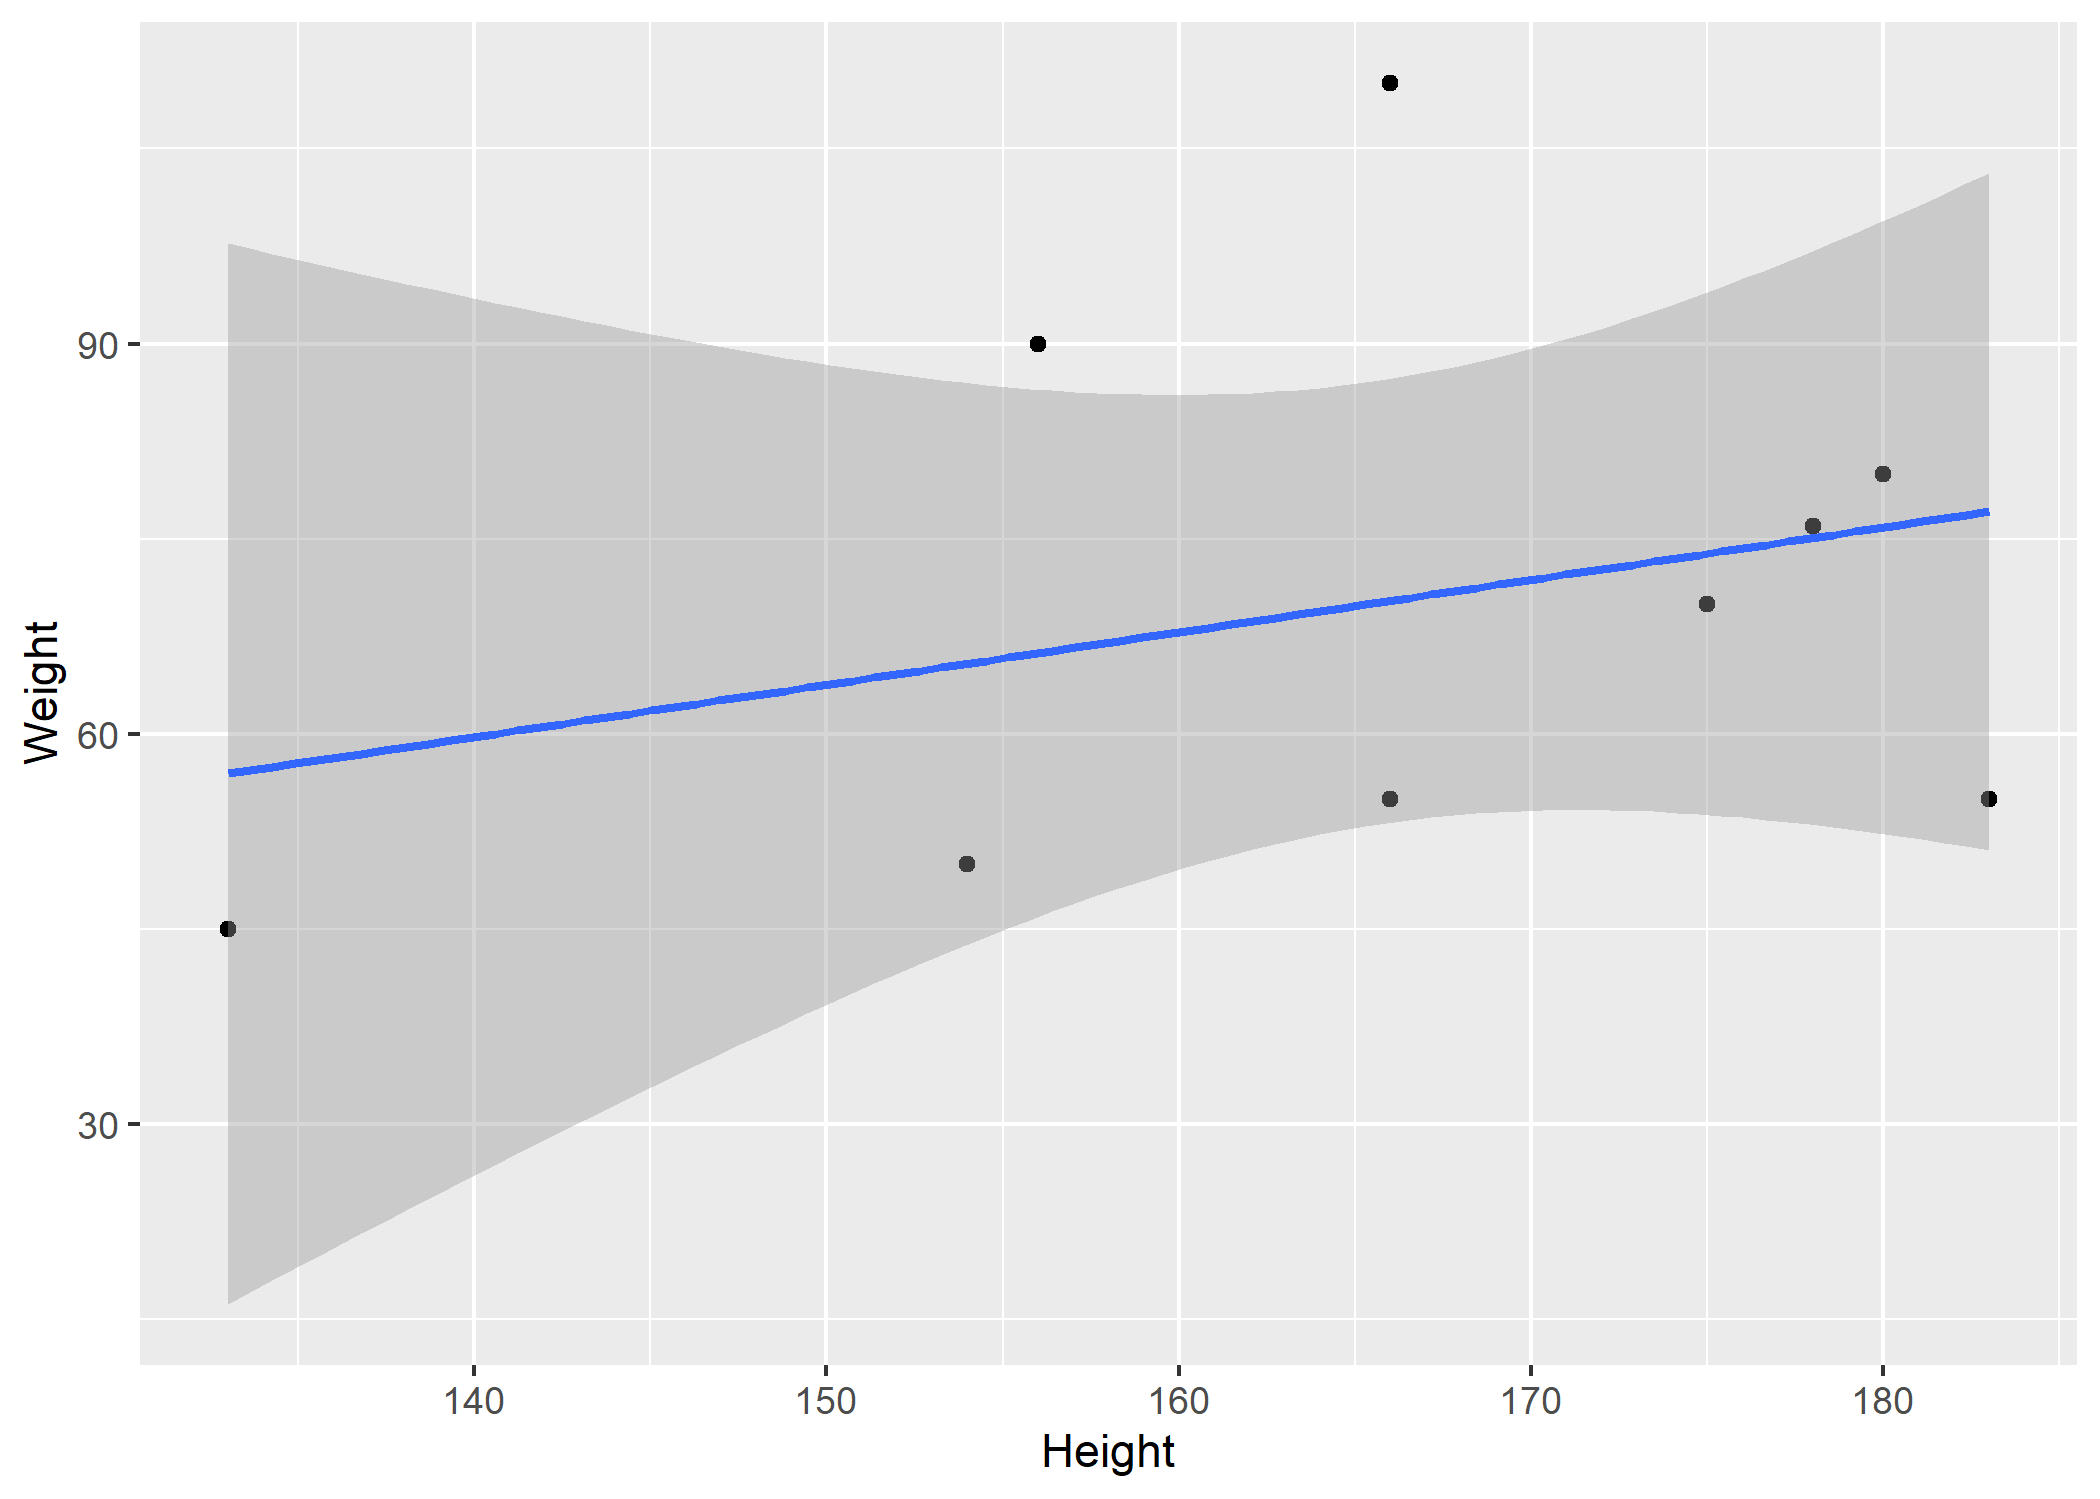
\includegraphics[width=7in,height=\textheight,keepaspectratio]{../../../results/figures/height-weight.png}

}

\caption{\label{fig-result2}Height and weight.}

\end{figure}%

~ ~

\subsection{Additional result}\label{additional-result}

\emph{Table 1: Regression Coefficients for the Association Between
Weight and Outcome}

\begin{longtable}[]{@{}lrrrr@{}}

\caption{\label{tbl-resulttable1}Another fit table.}

\tabularnewline

\toprule\noalign{}
term & estimate & std.error & statistic & p.value \\
\midrule\noalign{}
\endhead
\bottomrule\noalign{}
\endlastfoot
(Intercept) & 149.6997661 & 19.7518528 & 7.5790240 & 0.0001285 \\
Weight & 0.2277371 & 0.2708841 & 0.8407177 & 0.4282860 \\

\end{longtable}

~ ~

\section{Evaluating Discrimination (ROC Curve and
AUC)}\label{evaluating-discrimination-roc-curve-and-auc}

\emph{Additional Model Evaluation (Supplement)} Panel A shows the ROC
curve for the gravidity‐only logistic model in women under 25. The curve
lies modestly above the diagonal, reflecting fair discrimination (AUC ≈
0.55). Panel B is the corresponding calibration plot (decile‐based),
which compares observed event rates within probability bins to the ideal
45° line; slight deviations indicate some miscalibration in the highest
and lowest risk groups.

Panel C presents the bootstrap bias‐corrected calibration curve (200
resamples). The ``apparent'' (dotted) and ``bias‐corrected'' (solid)
lines both track closely to the ideal (dashed) reference, confirming
good overall calibration (mean absolute error ≈ 0.016). Panel D displays
the heatmap of cross‐validated AUC across the elastic‐net
penalty--mixture grid, illustrating that intermediate penalty values
(log₁₀λ around --2) and mixture α near 0.8 yielded the best
discrimination.

Finally, Table S7 reports the mean (±SE) cross‐validated ROC AUC for the
three machine‐learning algorithms: LASSO (0.55±0.012), random forest
(0.52±0.013), and XGBoost (0.497±0.014). This confirms that regularized
regression slightly outperformed the tree‐based methods under our tuning
scheme.

\emph{Supplementary Regression Coefficients (Table S8)} The simple
linear model of weight on height yields an intercept of 149.7g (SE 19.8,
p\textless0.001) and a non‐significant slope of 0.23g/cm (SE 0.27,
p=0.43), indicating that while taller women tended to weigh more on
average, this association was weak and did not reach statistical
significance in our sample.

~ ~

\emph{Figure S5: Calibration Plot: Gravidity Model (Age \textless{} 25)}

\begin{verbatim}
AUC: 0.58 
\end{verbatim}

\pandocbounded{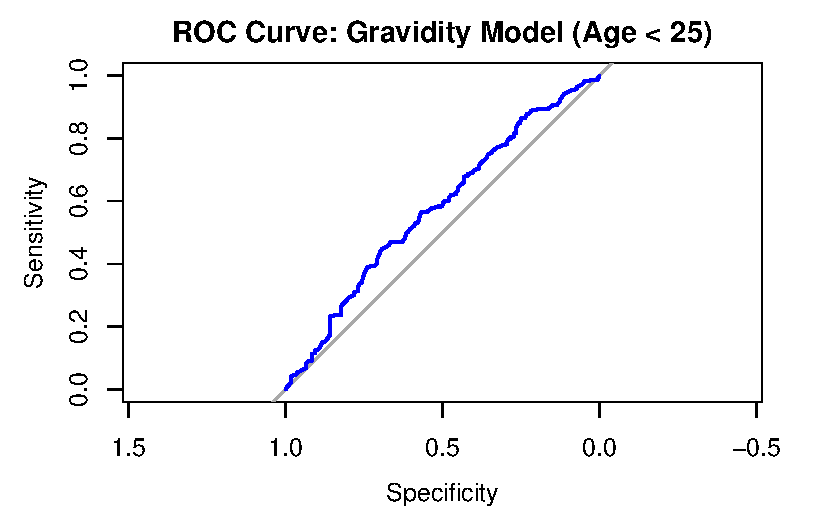
\includegraphics[keepaspectratio]{Supplementary-Material_files/figure-pdf/unnamed-chunk-9-1.pdf}}

\pandocbounded{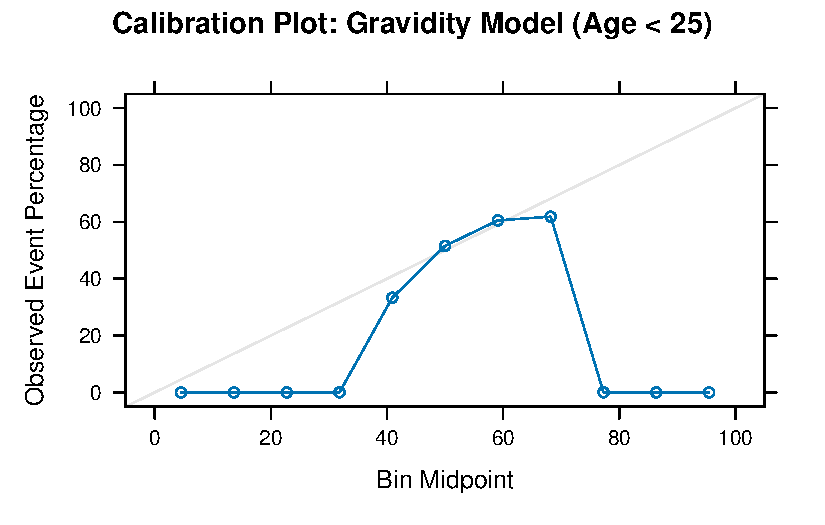
\includegraphics[keepaspectratio]{Supplementary-Material_files/figure-pdf/unnamed-chunk-9-2.pdf}}

~ ~

\textbf{Figure S6. Bootstrap‑calibrated calibration curve for the
malaria interaction model}

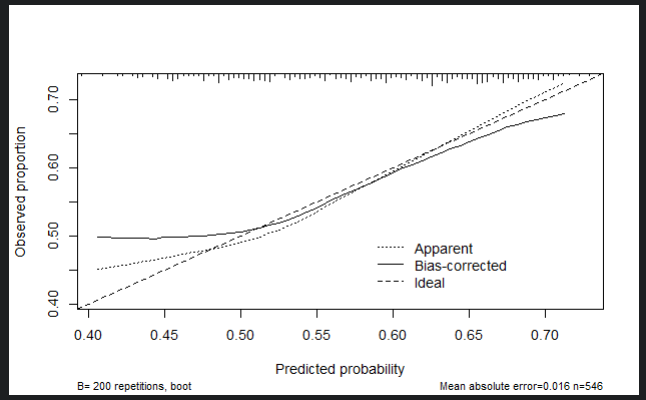
\includegraphics[width=2.15in,height=\textheight,keepaspectratio]{../Images/rms_model.png}

~ ~

\emph{Figure S7: Calibration curve for malaria interaction model in
women aged \textless25 years}

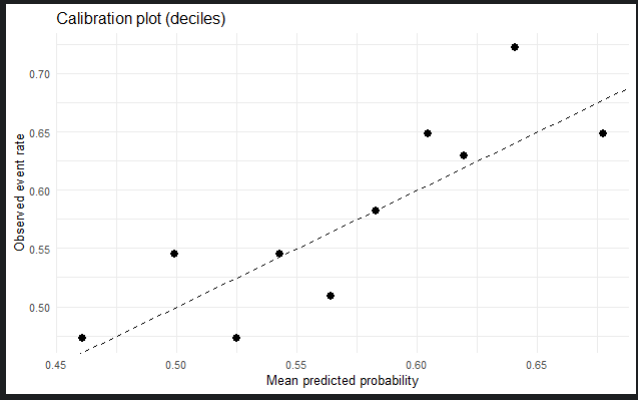
\includegraphics[width=2.13in,height=\textheight,keepaspectratio]{../Images/CalibrationPlot.png}

~ ~

\emph{Figure S8:Heatmap of five‑fold cross‑validated ROC AUC across the
elastic‑net penalty--mixture grid}

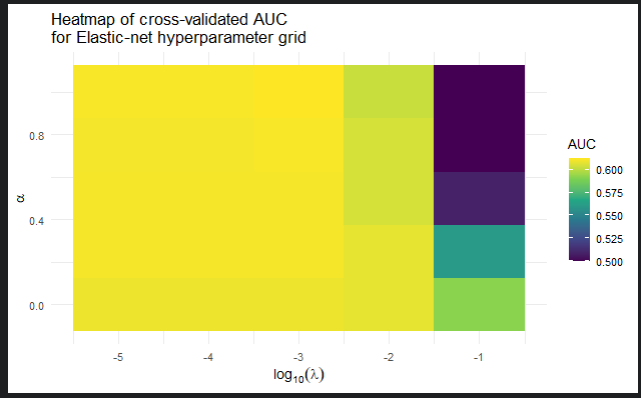
\includegraphics[width=2.14in,height=\textheight,keepaspectratio]{../Images/Heatmap.CV AUC.png}

~ ~

\emph{Table S2:Mean cross‑validated ROC AUC (±SE) for each
machine‑learning mode}

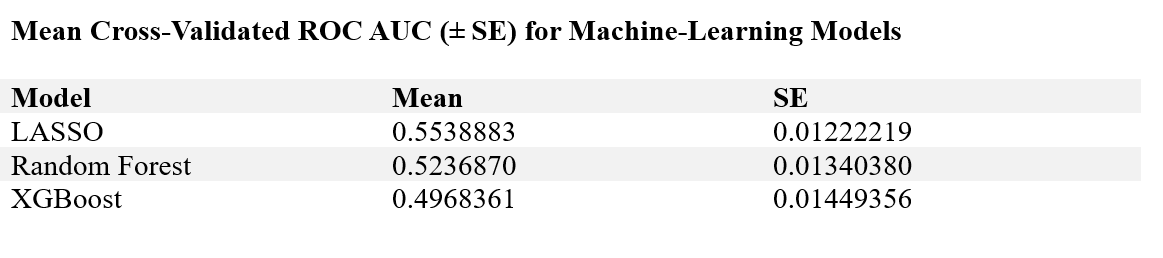
\includegraphics[width=3.88in,height=\textheight,keepaspectratio]{../Images/MeanCV ROC.AUC .png}

During 5‑fold cross‑validation, the elastic‐net model achieved the
highest mean AUC (0.55±0.01), followed by random forest (0.52±0.01) and
XGBoost (0.50±0.01).

\newpage{}

\section{Discussion}\label{discussion}

The supplementary materials deepen and validate our primary findings by
providing transparent documentation of all data‐processing steps,
extensive methodological details, and additional model diagnostics that
could not be accommodated in the main text. Detailed tables of
missingness, deviance tests, and variance inflation factors reinforce
the robustness of our interaction model. At the same time, the bootstrap
and decile‐based calibration curves confirm its reliability across risk
strata. The elastic‐net heatmap and cross‐validated AUC summaries for
LASSO, random forest, and XGBoost highlight that, under consistent
tuning, regularized regression offers the strongest discrimination in
our dataset. Exploratory bar charts of malaria episodes, gravidity, and
parity by treatment arm contextualize cohort characteristics, and the
gravidity‐only subgroup analyses (ROC and calibration plots) elucidate
how prior pregnancy history predicts adverse outcomes among younger
women. Together, these supplementary analyses enhance confidence in our
conclusions, demonstrate reproducibility, and offer a resource for
readers seeking to replicate or extend this work.




\end{document}
